\documentclass[a4paper,10pt,twocolumn]{article}

\usepackage[margin=0.85in]{geometry}
\usepackage[utf8]{inputenc}
\usepackage[T1]{fontenc}
\usepackage{
    lipsum,
    graphicx,
    float,
    cite,
    color,
    caption,
    hyperref,
    mathtools,
    fancyhdr,
    amsmath,
    amssymb,
    xparse,
    url
}

\hyphenpenalty=5000
\hypersetup{
  colorlinks=true,
  linkcolor=black,
  filecolor=magenta,      
  urlcolor=blue,
}

\renewcommand{\familydefault}{\sfdefault}

\date{}
\title{
    \small
    {\large Seminar in Mathematical Biology}\\
    Summer Semester 2024\\
    \vspace{1em}
    {\LARGE\bfseries Global AI Models for Multicellular Dynamics} \\ 
    {\Large Towards Learned Simulators for Cellular Migration}
}

\author{
    Paul-Lennard Zschoppe\footnote{4847097, paul-lennard.zschoppe@mailbox.tu-dresden.de}\\
    \and
    Syed Alisamar Husain\footnote{5198172, syed\_alisamar.husain@mailbox.tu-dresden.de}\\
}

\begin{document}
    \maketitle

    \begin{abstract}
        Spatiotemporal models are applied to study myriads of physical, chemical and biological
        phenomena, one of which is the problem of studying cellular dynamics.
        Global AI models are being applied to models that exhibit dynamics in spatial 
        and temporal domain. Successful applications of such neural simulators can be found in the 
        domains of physics, chemistry, and structural biology, amongst others. 

        In the presented work, the authors propose an autoregressive probabilistic model that can reproduce 
        spatiotemporal dynamics of single cell migration, traditionally simulated with the 
        Cellular Potts model. 
        According to them, a neural simulator for cellular dynamics can augment lab experiments and 
        traditional computational methods to enhance our understanding of a cell's interaction 
        with its physical environment. 
    \end{abstract}

    % one\cite{minartz_cpm}
    % two\cite{minartz_epns}
    % three\cite{morpheus}
    % three\cite{weng_autoencoders}
    % three\cite{rocca_vaes}


    \section{Cellular-Potts Model}
        Based on the earlier Potts Model, this is a computational model that can be used to study and simulate
        the motion and dynamics of cells and tissues. It is also used to simulate 
        individual and collective cell behavior, tissue morphogenesis and cancer development.
        
        The model consists of a rectangular {\bfseries Euclidean lattice} where each cell is a subset 
        of lattice sites sharing the same cell number. Lattice sites that are not occupied by 
        cells are the medium. 
        Consider function $x: L \to S$ that maps each lattice site $l_i$ to its state 
        $x(l_i) \in S$ where $S$ is the set of all cell numbers.

        \paragraph{Model Dynamics}
        The dynamics of the model are governed by an energy function $H$.
        At each iteration of the model a lattice site $l_i$ is chosen at random.
        Then, a proposal is made to modify $x$ such that state $x(l_i)$ is changed to 
        $x(l_j)$, where $l_j$ is a site adjacent to $l_i$.

        The difference in energy $\Delta H$ between the two states is calculated, by using the 
        energy function formulated as a Hamiltonian as in equation~\ref{eq:hamiltonian}.
        Difference in energy $\Delta H$ decides if the new proposed state is accepted.

        \paragraph{Energy Function}
        The original model proposed by Graner and Glazier\cite{cellular_potts} contains cells of two types, 
        with different adhesion energies for cells of the same type and cells of a 
        different type. Each cell type also has a different contact energy with the 
        medium, and the cell volume is assumed to remain close to a target value. 
        
        The Hamiltonian is formulated as:
        \begin{equation}
            \mathcal{H} = \sum_{i=0}^{n} \mathcal{J}(x(l_i), x(l_j)) + \sum_{i=0}^{n} \lambda_v {(V(c) - V^*(c))}^2
            \label{eq:hamiltonian}
        \end{equation}

        \begin{figure}[H]
            \centering
            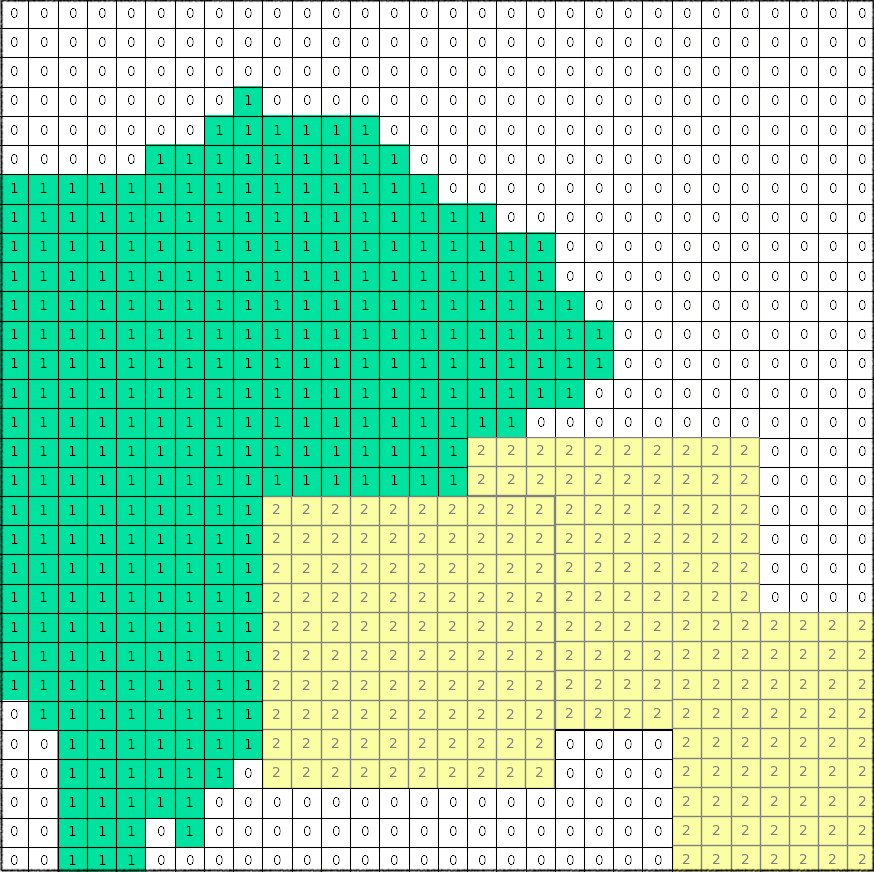
\includegraphics[width=0.49\textwidth]{../images/cpm_lattice.png}
            \caption{Euclidean Lattice of Cellular Potts model}\label{fig:cpm}
        \end{figure}

        If $\Delta H < 0$, the state is always accepted because systems tend to the lowest enegy state.
        But if $\Delta H > 0$, accepted with probability $e^{-\Delta H / T}$
        where $T$ is a parameter called Temperature.
        A higher temperature makes it more likely for higher enegy states to be accepted. 


    \section{Machine Learning Formulation}

        The authors utilize a machine learning model, based on the CVAE structure with 
        an additional so called forward model to interpret images\cite{minartz_cpm}. 

        \subsection{Autoencoders}
            The simple autoencoder is an architecture, with the 
            objective of encoding input data into a latent representation only 
            containing core features and aspects of the original input\cite{weng_autocoders}.
            
            \begin{figure}[H]
                \centering
                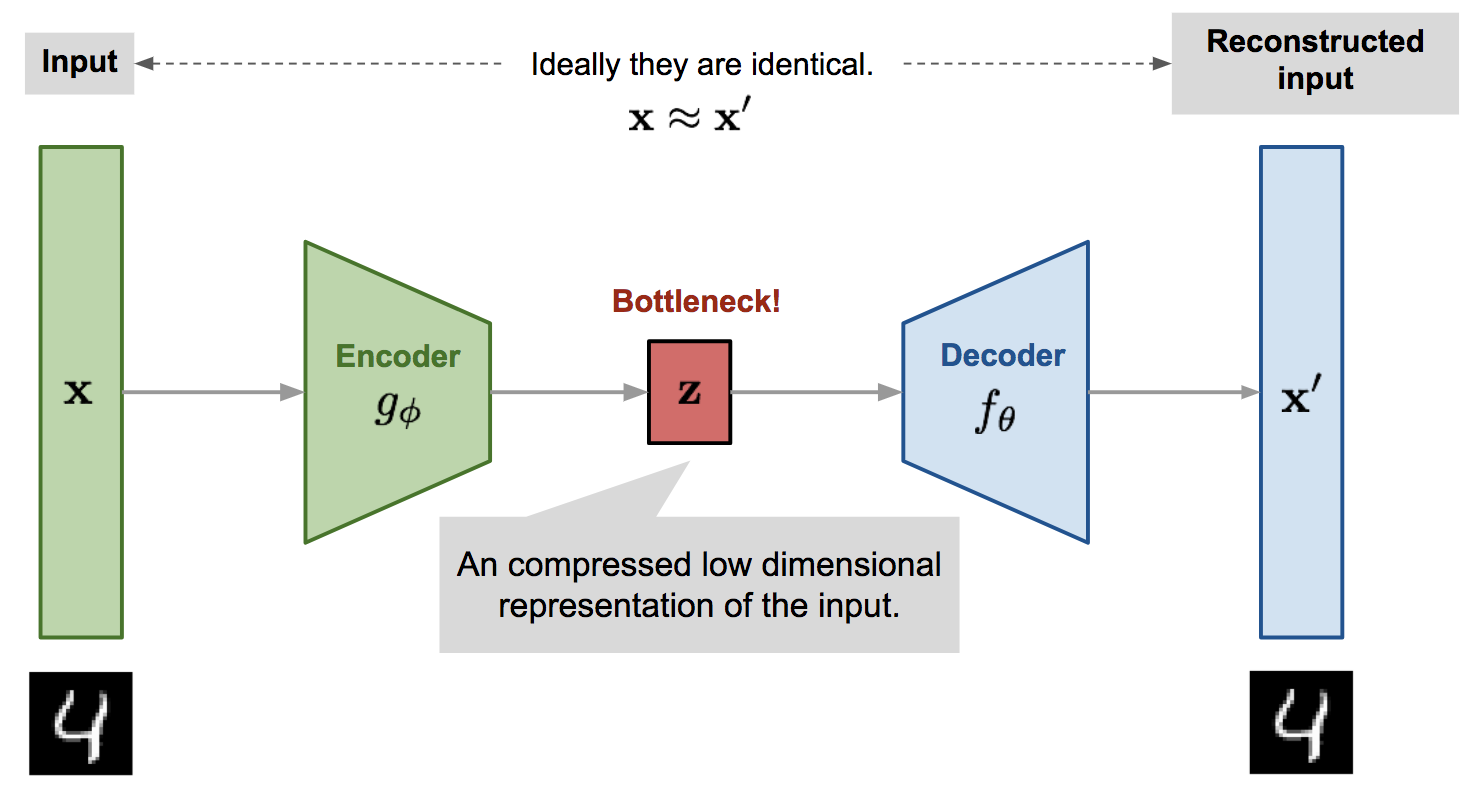
\includegraphics[width=0.49\textwidth]{../images/autoencoder-architecture.png}
                \caption{Autoencoder Architecture}\label{fig:autoencoder}
            \end{figure}

            To achieve this, we optimize parameters of encoder $g_{\theta} ({x_n})$ 
            encodes a high dimensional input $X$ into a lower dimensional latent space $z$ 
            and the parameters of decoder $f_{\phi} (g_{\theta} ({x_n}))$ which reconstructs it into $X'$,
            such that the reconstruction is lossless.

            \begin{equation}
                \mathcal{L}_{\phi, \theta}({x}, {x'}) = \frac{1}{N} \sum_{n=1}^{N} {({x_n} - f_{\phi} (g_{\theta} ({x_n})))}^2
                \label{eq:lossfunc}
            \end{equation}
            
            \paragraph{Variational Autoencoders}
            Instead of mapping the input space $X$ into a fixed vector, variational autoencoders
            map it into a distribution $p_\theta$ parameterized by $z$\cite{rocca_vaes}.
            This makes it possible to sample the latent space to get samples that are a combination
            of two entities in the input space.
            To train VAEs, the Evidence Lower Bound (ELBO) loss function can be used.

            \paragraph{Conditional Variational Autoencoders}
            Whereas the simple autoencoder formulates the latent representation as the probability of
            $z$ given $X$, conditional variational autoencoder adds just an additional conditional variable, 
            with encoder $p_\theta (z | X, c)$, and decoder $q_\phi (X | z, c)$\cite{cvaes}.

            \begin{figure}[H]
                \centering
                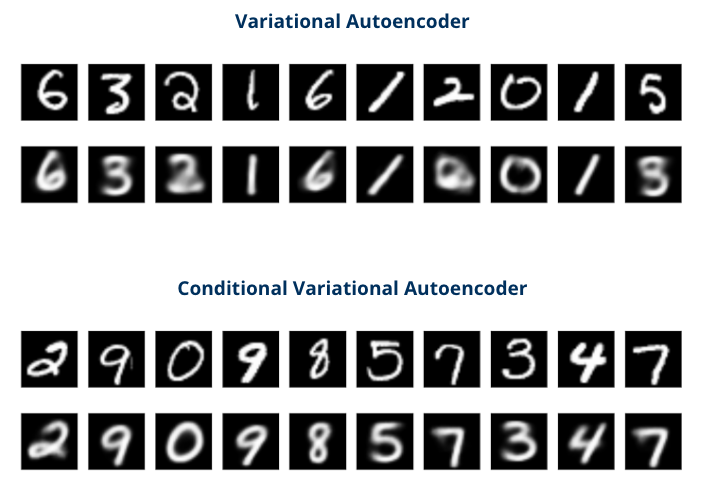
\includegraphics[width=0.49\textwidth]{../images/vae_vs_cvae.png}
                \caption{Improved reconstructed images with CVAEs}\label{fig:vae_vs_cvae}
            \end{figure}


        \subsection{Modelling Cellular-Potts}
            At each time $t$ the system is described by its state $x^t$, a
            categorically-valued function on a fixed grid. 
            Correspondingly, a system evolution is specified by a sequence of states $x^{[0:T]}$.
            The authors postulate a ground-truth probability distribution $p_*(x^{[0:T]})$\cite{minartz_cpm} 
            over system evolutions $x^{[0:T]}$ from which we can sample using the CP simulator. 
            
            Hence, our aim is to learn the parameters $\theta$ of the model $p_\theta$ to maximize:
            \begin{equation}
                \mathbb{E}_{t \sim U_{\{0,T-1\}}} \mathbb{E}_{x^t \sim p_*} \log p_\theta(x^{t+1} | x^t)
            \end{equation}

            This is achieved with a conditional variational autoencoder, where latent variable 
            $z$ is conditioned on previous state $x^t$ according to conditional prior
            $p_\theta(z|x^t)$ and the subsequent state $x^{t+1}$ follows the 
            distribution $p_\theta(x^{t+1} | x^t, z)$.

            \begin{figure}[H]
                \centering
                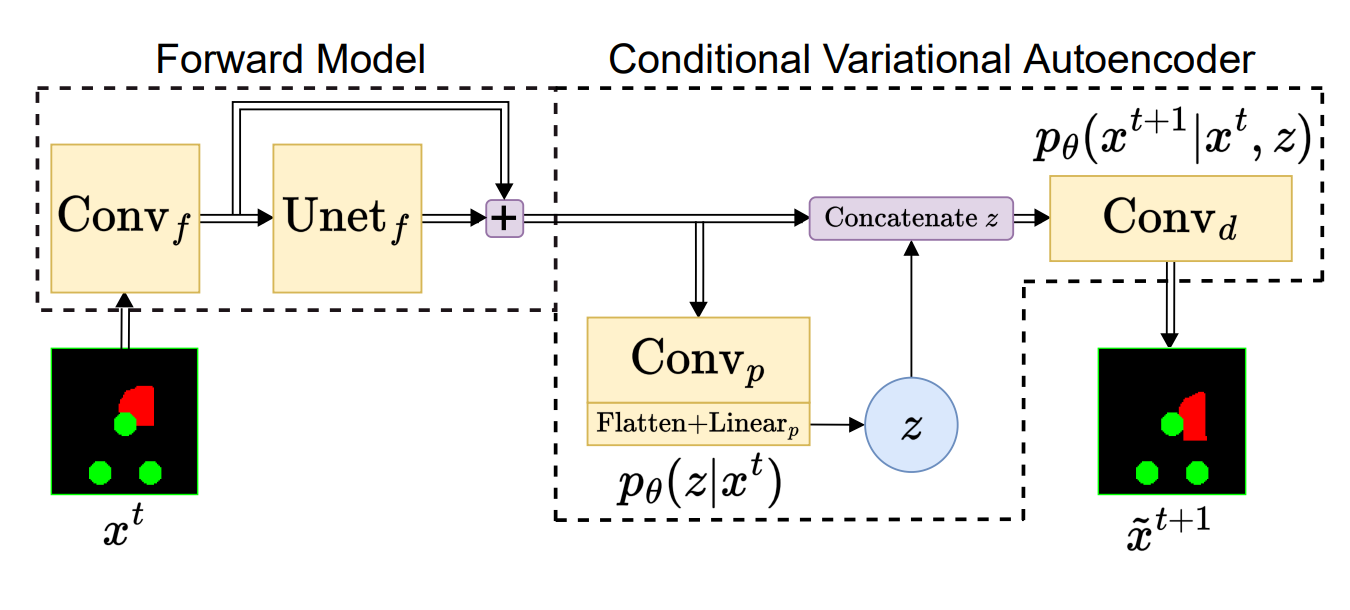
\includegraphics[width=0.49\textwidth]{../images/architecture.png}
                \caption{Model Architecture}\label{fig:architecture}
            \end{figure}

            As this model is an autoregressive model, it consists of a forward model that evolves the state of
            the system to the next state. However, rather than directly producing the pixel-wise parameters of a
            distribution to sample the next state from, the representation produced by the forward model is used
            to first condition the prior distribution of the latent variable. Then, to produce a sample of the next
            state, the latent variable is sampled from this prior and combine it with the forward representation,
            which is subsequently decoded.

            \begin{equation}
                L_{\phi, \theta} = -D_{KL}(q_\phi || p_\theta)
                + \mathbb{E}_{q_\phi}[\log p_\theta(x^{t+1}|x^t, z)]
                \label{eq:elbotrain}
            \end{equation}
            
            During training, the Evidence Lower Bound (ELBO) on the log-likelihood (equation~\ref{eq:elbotrain})
            is optimized. During trajectory generation we sample latent variable $z$ from the prior 
            distribution $p_\theta(z | x^t)$.
            
            By then sampling $\tilde{x}^{t+1} \sim p_\theta(x^{t+1}|x^t, z)$ and
            repeating the entire process, we can simulate longer trajectories.


    \section{Training and Analysis}
        We train our own version of the model proposed by paper since, to our knowledge, 
        a pre-trained model is not publically avaiable yet. We have modified the original
        code published by the authors to able to do this. 
        Our code is also available on Github\footnote{\url{https://github.com/zrthxn/EPNS}}.

        \paragraph{Dataset}
        To generate training samples we have used a Morpheus\footnote{\url{https://morpheus.gitlab.io/}}\cite{morpheus} 
        model for Cellular-Potts.
        We generated initial conditions with random stationary walls and one cell and two cells. 
        This gives us two datasets, each eith 800 training samples, 100 validation and test samples.
        
        \paragraph{Training}
        We trained two models using the aforementioned two datasets, using one NVIDIA A100 
        provided by HPC at ZIH, TU Dresden.

        \subsection{Results and Analysis}
            We run the models on the test split of both of the datasets that we generated.
            Both models, one and two cells, are tested with both datasets.

            \begin{figure}[H]\centering
                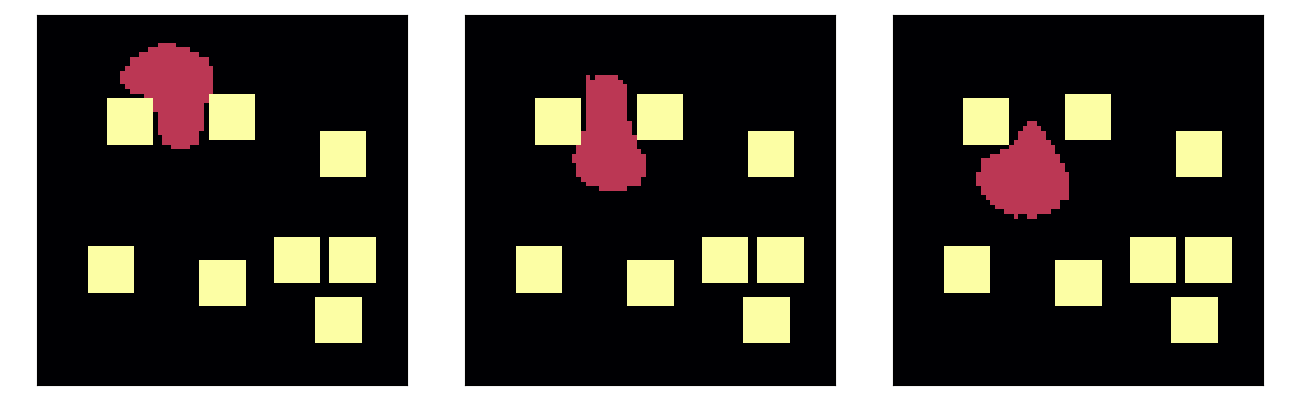
\includegraphics[width=0.49\textwidth]{../images/run_40.png}
                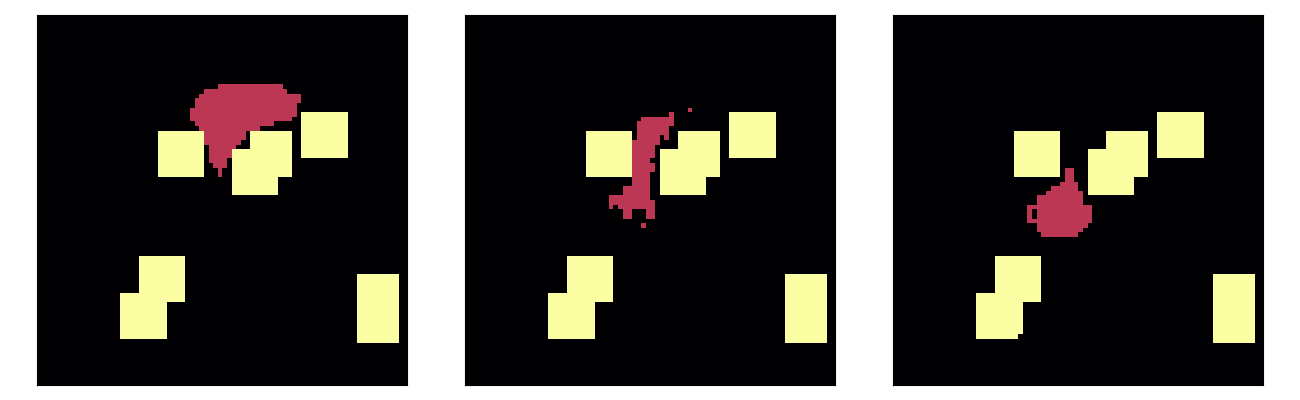
\includegraphics[width=0.49\textwidth]{../images/run_32.png}
                \caption{Neural Simulator: Dynamics of One Cell}
            \end{figure}
            The model is able to learn the expected dynamics of the cells.
            However we sometimes see gaps and holes
            in the cells, as well as some movement of the walls.

            \begin{figure}[H]\centering
                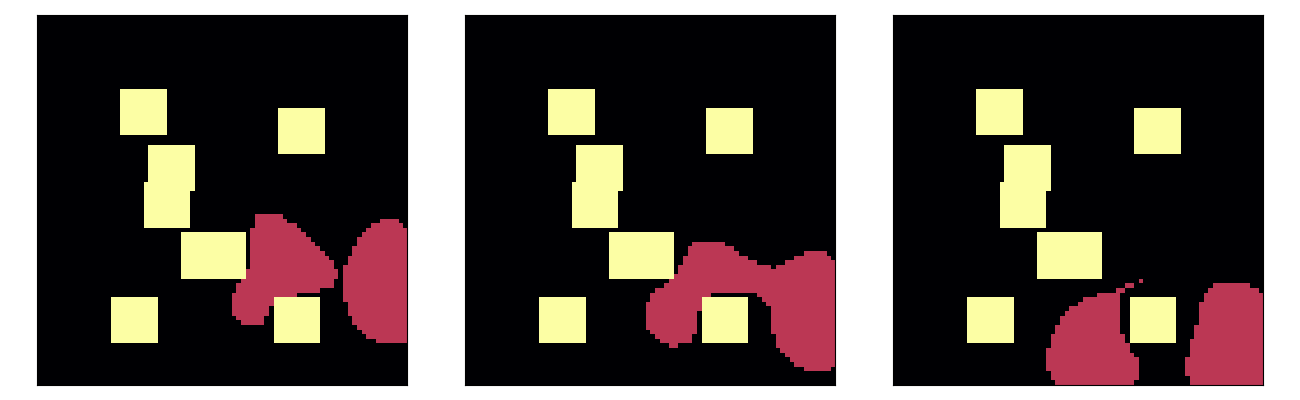
\includegraphics[width=0.49\textwidth]{../images/run_22.png}
                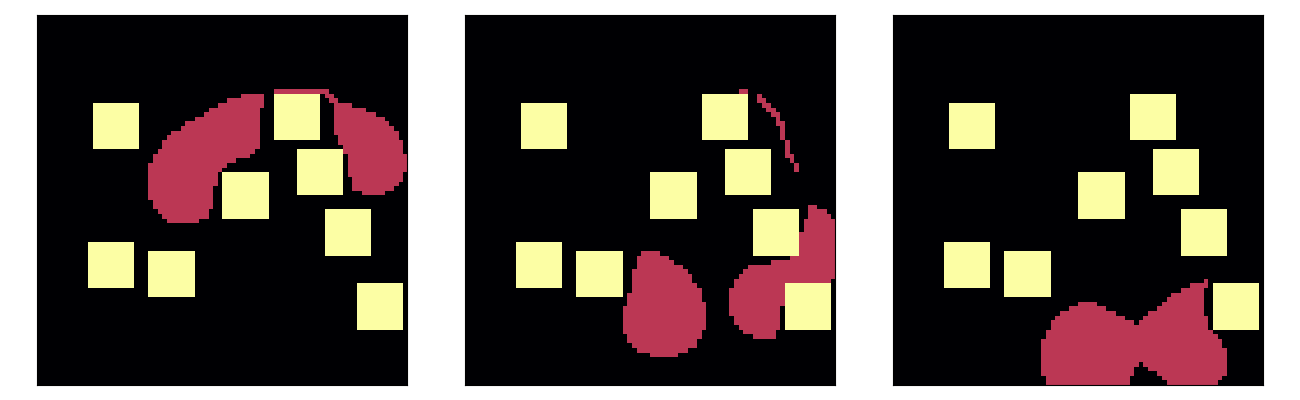
\includegraphics[width=0.49\textwidth]{../images/run_12.png}
                \caption{Neural Simulator: Dynamics of Two Cells}
            \end{figure}
            Similarly we see expected output from the two-cell model. We also see that the
            single-cell model is able to transfer to the two-cell cases.
            
            \paragraph{Edge Cases}
            We have also seen some edge cases where the model breaks down.
            Sometimes we can see gaps and holes in the cells, as well as some movement of the walls.
            Also, the cells sometimes lose volume and disappear.
            \begin{figure}[H]\centering
                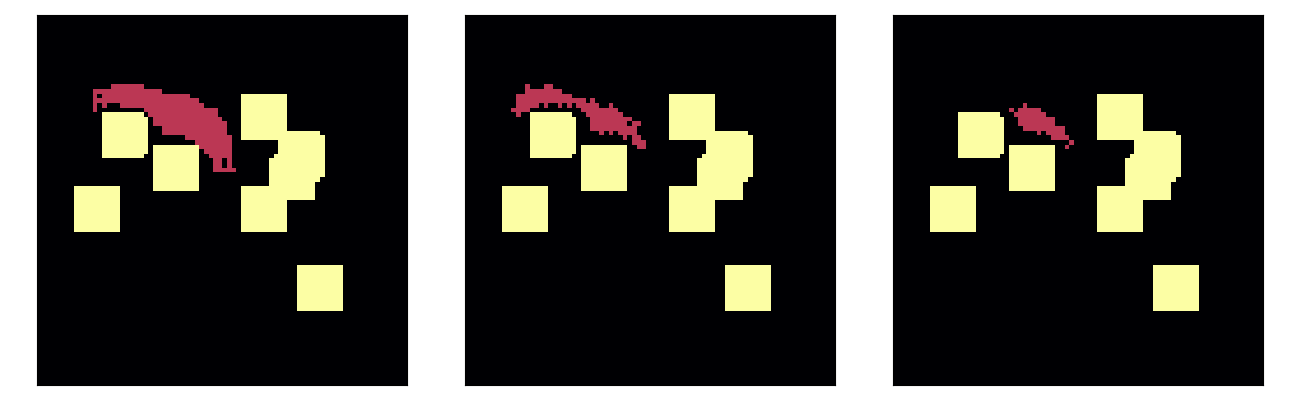
\includegraphics[width=0.49\textwidth]{../images/run_5.png}
                \caption{Edge Cases: Destruction of volume}
            \end{figure}

    \section{Conclusion}
        We conclude that the problem of predicting cell motility is non-trivial, and that
        the architectural choices for the machine learning model are well suited to the problem.
        Edge cases, while present, are rarely observed.

        Applications to real-world microscopy data are possible with minimal changes to the model.
        Explainability analysis may help understand how cells decide their motility.
        Most notably, this approach bypasses the need for a mechanistic understanding of the system.

        \subsection*{Contributions}
            Review of the paper was done collaboratively. 
            To produce the results shown, Paul worked on data generation and Ali on model training.
            Both authors contributed equally to presentation slides and this article.

    
    \bibliographystyle{ieeetr}
    \bibliography{./references}

\end{document}